\section{Datasets and crawling methodology} 
\label{sec:4_3_methodology}

%FLEET OF CS systems
This work relies on usage data from three car-sharing services: Modo, Car2Go, and Evo. These services operate in several cities and countries. We focus on data from the Vancouver area, where all these three services operate. Modo fleet is composed of combustion, electric and hybrid cars; Car2go offers combustion cars and finally, Evo supplies only hybrid vehicles. For each service, we collected both users' trips and fleets composition. In total, we observed more than 680 cars for Modo, 1\,200 for Car2go, and 1\,000 for Evo.

% DATA COLLECTION
For all the three services, we collected vehicle status minute-by-minute, through public Application Programming Interfaces (APIs) or, directing accessing their service information web-page. From those requests it is possible to scrape also an unique ID and position of each car present in the dataset. In short, through the Modo API\footnote{Modo API, \url{http://modo.coop/api/}} returns the station and vehicle IDs. Modo provides vehicles status too: a car indeed may be available, reserved or running.
Evo's data\footnote{Evo public portal, \url{https://www.evo.ca/api/Cars.aspx}} information page allow to check the remaining vehicle fuel (in percentage) and its location. Finally, Car2go APIs\footnote{Car2go API, \url{https://www.car2go.com/api/tou.htm }, last access February 2018}. 
Data from Evo and Modo comprises five months, ranging from March 1st, 2018 to July 16th, 2018. Car2Go data comprises thirteen months, ranging from  December 31st, 2016 to January 31st, 2018. It is important to notice that, to not violate the users' privacy, the providers do not expose any users' personal information. Moreover, the companies do not track the cars during a trip so we do not know exactly the travel path, but only the start/end positions and the duration of travel.

All measurements used in our analyses are publicly available the following trace repository:
\url{http://netlab.ice.ufjf.br/index.php/carsharingdata/}


\subsection{Modo crawling methodology and data summary}


%MODO data collection
The Modo data collection process was conducted with a crawler that uses its public API. 
First, we request to the Modo API the list of all vehicles of the service. 
Then, minute by minute, we request the status of each of these vehicles. Each request returns the schedule of a vehicle, informing the periods it will be available for the next 24-hours. Moreover, it returns the vehicle location, i.e., the station with its identifier. 
Note that Modo API does not return specific vehicle status, nor any information that could be used to identify users of the system. We uncover if a vehicle is busy or idle based on its reservation period and the current observation time. In other words, we collect several vehicle schedules and compare each other. Figure~\ref{fig:4_3_capturas} illustrates the process of collecting data for a given vehicle. Each data sample corresponds to a request to the API in the order they occur. Data sample \#1 is the result of the API request at minute 1 ($t=1$), data sample \#2 is the result of the API request at minute 2 ($t=2$), etc. At each data sample, the blue dot represents the time a vehicle will be available. We highlight three possible situations:

\begin{itemize}
\item First, as shown in figure~\ref{fig:4_3_capturas}(a), at $t=1$ a given vehicle is shown reserved up to $t=5$.  At $t=2$, the new request to the Modo API still show us that the vehicle will be available only at $t=5$. Each of the following requests to the API confirms the booking period. At the time $t=6$, we perform a request to the API and the vehicle is no longer booked. In sum, we are able to infer that someone booked the vehicle before or at $t=1$, and returned it to the station at $t=5$.

\item Second, as shown in figure~\ref{fig:4_3_capturas}(b), at $t=1$  the Modo API returns that a given vehicle is reserved up to $t=6$.  However, in this case, a request at $t=5$ shows the vehicle is no longer reserved. In this case, we can infer that the user returned the vehicle earlier to the station which means she/he used the vehicle only up to $t=5$.

\item Finally, as shown in figure~\ref{fig:4_3_capturas}(c), the user may extend the booking period. More precisely, at $t=1$ the given vehicle is reserved up to $t=5$. At the third request, we note that the vehicle will no longer be available at $t=5$ but $t=6$. The following API requests confirm the use of the car until $t=6$.
\end{itemize}


\begin{figure}[!htb]
	
      \centering
      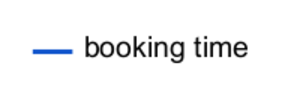
\includegraphics[height=1cm]{modo_methodology/time.pdf}
   	  \quad 
      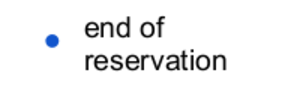
\includegraphics[height=1cm]{modo_methodology/point.pdf}
 

    \medskip
    
    \begin{minipage}[b]{0.32\columnwidth}
    \centering
     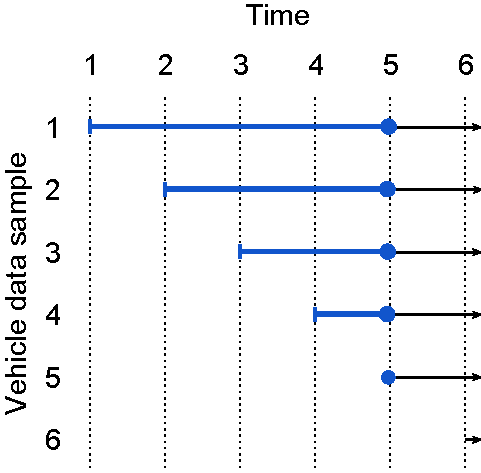
\includegraphics[width=\linewidth]{modo_methodology/Normal_Situation.pdf}
     {\\(a) Normal \\situation}
    \end{minipage}
    % \hspace{5mm}
    \begin{minipage}[b]{0.32\columnwidth}
     \centering
     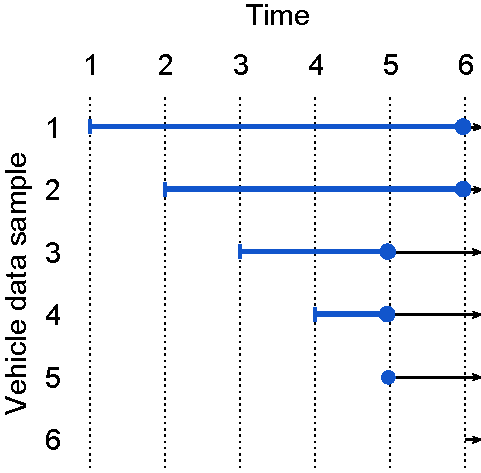
\includegraphics[width=\linewidth]{modo_methodology/Cancelation_Situation.pdf}
    %  \vspace*{-3mm}
     {\\(b) Anticipated vehicle return}
    \end{minipage}
    %\hspace{1cm}
    %\hspace{5mm}
    \begin{minipage}[b]{0.32\columnwidth}
    % \vspace{5mm}
     \centering
     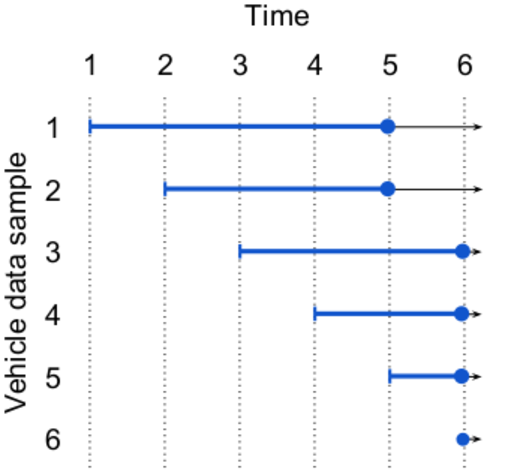
\includegraphics[width=\linewidth]{modo_methodology/Consecutive_without_legend.pdf}
     {\\(c) Extended travel situation}
    \end{minipage}
    \caption{Possible vehicle status during the Modo crawling. In (a) a normal booking and usage situation; (b) a cancellation situation; (c) a consecutive booking situation.}
    \label{fig:4_3_capturas}
\end{figure}

Besides, we also collect base stations location, vehicle models and whether the vehicle is electric or hybrid. 
Table~\ref{table:4_3_dataModo} summarizes the data we have collected from Modo. We stored 134 millions of records in 5 months, from a fleet of 682 vehicles distributed in 528 stations, each of them with one or more cars. The stations are located in Vancouver, Canada, and its neighbor cities. This data allows us to analyze more than %149 thousands of booking records and 
98\,000 travels.\footnote{Data are available on http://netlab.ice.ufjf.br/index.php/carsharingdata/}
% \footnote{Data will be available for researchers upon request.}

\begin{table}[tbh]
	\setlength{\tabcolsep}{2.3pt}
	\centering
		\begin{tabular}{llr}
		%\multicolumn{2}{l}{Description}                     & Amount \\ 
		\hline
		\multicolumn{2}{l}{\# of Collected Records}  & $\approx$ 134\,000\,000\\
		\multicolumn{2}{l}{\# of Booking Records} & 149\,732  \\
		\multicolumn{2}{l}{\# of Travels Records} & 98\,915   \\
		\multicolumn{2}{l}{\# of Stations} & 528    \\\hline   
		\multirow{3}{*}{\# of Vehicles}       & - Common    & 530 \\
		                                      & - Hybrids  & 148 \\
		                                      & - Electrical & 4 \\
		                                      \hline
		\end{tabular}
	\caption{Summary of the Modo dataset.}
	\label{table:4_3_dataModo}
\end{table}


%%%%%%%%%%%%%%%%%%%%%%%%%%%%%%%%%%%%%%%%%%%%%%%

\subsection{Evo crawling methodology and data summary}

Evo does not offer a public API to researchers. For this reason, we collect data which is publicly available at its web portal. Minute by minute, we retrieve a list of all system vehicles. Moreover, we request service snapshots, describing which vehicles are parked, where they are parked and if they are available to travel. 
We process all snapshots of the system to infer the moments a vehicle is busy (rented) or idle (parked at a station). During a snapshot, if a vehicle is listed among the system vehicles but it is not parked at any station, we infer it is in use. Then, we set-up the travel starting point as the last station the vehicle was parked. Analogously, the travel ending point will be the next station the vehicle appears in a future snapshot. The total travel time is accounted for as the difference between these snapshots times. 
For each travel we identify, we also record the end-to-end path, according to the Google Maps API. In this way, we are also able to calculate the estimated travel, taking into account the local traffic conditions. Clearly, this estimation does not take into account the car-sharing client behaviour and, as a consequence, differ from the real travel time we also store. 
One may reserve a car in Evo and cancel this reservation, within a thirty minutes range, without any charges. Thus, we infer the number of cancellation in Evo by filtering short travels (i.e., $<$ 30 minutes) where the start and end points are the same. To accommodate GPS imprecision, we consider a 3~meters threshold. 
Table~\ref{table:4_3_dataEvo} summarizes the data we collect from Evo.
%In short, we collected more than 10 million records and 1 million travels, of a fleet with more than a one thousand vehicles and 130 stations. 
Note that this service does not need a large number of stations because the user can park the car in some public park spots in the service area, that is called home zone (Vancouver and its neighbor cities).

\begin{table}[htb]
\centering
\setlength{\tabcolsep}{2.3pt}

\begin{tabular}{llr}
%\multicolumn{2}{l}{Description} & Amount\\ 
\hline
\multicolumn{2}{l}{\# of Collected Records} & 142\,853\,500
\\
\multicolumn{2}{l}{\# of Travels Records} &  644\,887\\
%1\,232\,262\\
\multicolumn{2}{l}{\# of Stations}  & 130  \\\hline
\multicolumn{2}{l}{\# of Vehicles} & 1\,237
%1\,003 
\\\hline
\end{tabular}
\caption{Summary of the Evo data collection.}
\label{table:4_3_dataEvo}
\end{table}

\subsection{Car2Go crawling methodology and data summary}
\label{ss:4_5_datacollect}
 
The car2go data collection is widely described in chapter \ref{chap:2_datacollection}. 
%In a nutshell, car2Go offers APIs providing information about available cars at the moment of the request. Each API request returns, among other information, the car unique ID, its position and other fields which specifically describe the car status. Therefore the API response is semantically equivalent to the Evo's one. In this way, we applied the same methodology to gather and store the Car2go data too.

Recalling that the software is able to detect two events, corresponding to the car status change, clearly observable from the data. Indeed considering the current time instant $t_i$: 
\begin{itemize}
     \item if in $t_i$ the car is present in the API response and at time $t_{i+1}$ it is not, that car passes from available to rented. %It represents a parking event finish and a booking.
     \item if in $t_i$ the car is \emph{not} present and at time $t_{i+1}$ it reappears in the API reply, that car passes from rented  to available. It represents a booking finish and a parking beginning.  Indeed, for privacy constraints, the position of the car during a booking is not available.
\end{itemize}

%Notice that from a single rented status is impossible to estimate the travelled distance: by computing the Euclidean or Haversine 
%distance it is possible to deduce a lower bound of the real travel distance which is practically too optimistic to be used as a primary travel estimation. To improve this estimation we attach to each entry the distance provided by the Google Maps API. 
%As in Evo's methodology, we infer the number of cancellations by filtering short travels where the start and end points are very close.
Notice that, the straight distance (computed with the Haversine formula) between the ride starting and final points it is not the real driven distance hidden for privacy issues. For this reason the software attaches for each ride the distance provided by the Google Maps API, in order have a better estimation of the driven pattern. 

 Table~\ref{table:4_3_dataCar2Go} summarizes Car2go dataset. We have more than one million travels in thirteen months of data. As a free-floating service, Car2Go does not have stations but it has an operation zone, that covers a large area of Vancouver city and North-Vancouver. 

\begin{table}[htb]
	\centering
	\setlength{\tabcolsep}{2.3pt}
	\begin{tabular}{llr}
	%\multicolumn{2}{l}{Description} & Amount\\ 
	\hline
	\multicolumn{2}{l}{\# of Travels Records} & 1\,095\,577\\
	%1\,340\,053\\
	\multicolumn{2}{l}{\# of Vehicles} & 1\,077
	%1\.273 
	\\\hline
	\end{tabular}
	\caption{Summary of the Car2Go data collection.}
	\label{table:4_3_dataCar2Go}
\end{table}